%%%%%%%%%%%%%%%%%%%%%%%%%%%%%%%%%%%%%%%%%%%%%%%%%%%%%%%%%%%%%%%%%%%%%%%%%%%%%%%
% Definici\'on del tipo de documento.                                           %
% Posibles tipos de papel: a4paper, letterpaper, legalpapper                  %
% Posibles tama�os de letra: 10pt, 11pt, 12pt                                 %
% Posibles clases de documentos: article, report, book, slides                %
%%%%%%%%%%%%%%%%%%%%%%%%%%%%%%%%%%%%%%%%%%%%%%%%%%%%%%%%%%%%%%%%%%%%%%%%%%%%%%%
\documentclass[a4paper,10pt]{article}


%%%%%%%%%%%%%%%%%%%%%%%%%%%%%%%%%%%%%%%%%%%%%%%%%%%%%%%%%%%%%%%%%%%%%%%%%%%%%%%
% Los paquetes permiten ampliar las capacidades de LaTeX.                     %
%%%%%%%%%%%%%%%%%%%%%%%%%%%%%%%%%%%%%%%%%%%%%%%%%%%%%%%%%%%%%%%%%%%%%%%%%%%%%%%

% Paquete para inclusi\'on de gr\'aficos.
\usepackage{graphicx}

\usepackage{enumerate}

% Paquete para definir la codificaci\'on del conjunto de caracteres usado
% (latin1 es ISO 8859-1).
\usepackage[latin1]{inputenc}

% Paquete para definir el idioma usado.
\usepackage[spanish]{babel}

\usepackage{multirow} 

% Paquete para f\'ormulas matem\'aticas
\usepackage{amsmath}

% Espacio luego de titulos
\usepackage{titlesec}

\newcommand{\BigO}[1]{\ensuremath{\operatorname{O}\bigl(#1\bigr)}}

%\titleformat{hcommandi}[hshapei]{hformati}{hlabeli}{hsepi}{hbefore-codei}[hafter-codei]
\titlespacing\subsection{5pt}{12pt plus 4pt minus 2pt}{12pt plus 2pt minus 2pt}
\titlespacing\subsubsection{10pt}{0pt plus 2pt minus 2pt}{0pt plus 2pt minus 2pt}

\usepackage{listings}

\usepackage{fancyhdr}
\pagestyle{fancy}
\fancyhead{} % clear all header fields
\renewcommand{\headrulewidth}{0pt} % no line in header area
\fancyfoot{} % clear all footer fields
\fancyfoot[LE,RO]{\thepage}           % page number in "outer" position of footer line
\fancyfoot[RE,LO]{Entrega 1} % other info in "inner" position of footer line

%\usepackage{multicolumn} 

% T\'itulo principal del documento.
\title{		\textbf{Trabajo pr\'actico}}

% Informaci\'on sobre los autores.
\author{	Alejandro Garc\'ia Marra, \textit{Padr\'on Nro. 91.516}                     \\
            \texttt{ alemarra@gmail.com }                                              \\
            Sebasti\'an Javier Bogado, \textit{Padr\'on Nro. 91.707}                     \\
            \texttt{ sebastian.j.bogado@gmail.com }                                              \\
            \normalsize{1er. Cuatrimestre de 2013}                       \\
            \normalsize{71.14 Modelos y Optimization I}                             \\
            \normalsize{Facultad de Ingenier\'ia, Universidad de Buenos Aires}            \\
       }
\date{}




\begin{document}

% Inserta el t\'itulo.
\maketitle

% Quita el n\'umero en la primer p\'agina.
\thispagestyle{empty}


\newpage
\section{Ejercicio Principal}

\subsection{An\'alisis del caso}

En esta situaci\'on problem\'atica, nos encontramos con una refiner\'ia de petr\'oleo, la cual elabora distintos productos finales, compuestos por diversos sub-productos. Lo que se busca entonces es optimizar las ganancias obtenidas por los productos finales, por medio de la correcta distribuci\'on de los sub-productos en los procesos intermedios.

\subsection{Objetivo}
Determinar la cantidad de barriles de los distintos tipos de combustible, fueloil y lubricante a producir, as\'i como la composici\'on de los combustibles para maximizar las utilidades de la refiner\'ia por d\'ia.
\vspace{10mm}

\subsection{Hip\'otesis y Aclaraciones}

\begin{itemize}
 \item {Precio constante en el d\'ia}
 \item {No tengo stock inicial}
 \item {Se vende todo lo producido y, por ende, se puede hablar de fracciones de barril}
 \item {Se dispone de dinero suficiente para comprar toda la materia prima necesaria}
 \item {Puedo comprar cantidades fraccionarias de la materia prima}
 \item {Las m\'aquinas no se rompen ni los empleados se rebelan}
 \item {Al hablar de ``barriles'' para refererirse a cantidad, un barril de un producto es igual al de otro}
 \item {No hay perdidas de producci\'on ni transporte, excepto las indicadas en la destilaci\'on}
 \item {En las mezclas no se agrega nada que no est\'e mencionado, entonces las proporciones deben sumar 1}
 \item {El centro de destilaci\'on puede alternar entre crudo de tipo 1 y tipo 2 sin p\'erdidas de tiempo o costos adicionales. Lo mismo aplica para el centro de reformado y craqueo respecto de sus distintas entradas}
 \item {A menos que se indique lo contrario, puede no producirse alguno de los productos finales}
 
 
 
\end{itemize}
	
\newpage

\subsection{Variables}


\subsubsection{Compra}
\vspace{5mm}

$C1 = $ Barriles de Crudo 1 por d\'ia \\

$C2 = $ Barriles de Crudo 2 por d\'ia \\
\vspace{2mm}

\subsubsection{Destilado}
\vspace{5mm}

$NL = $ Barriles de Nafta Liviana por d\'ia \\

$NL^{REF} = $ Barriles de Nafta Liviana para Reformado por d\'ia \\

$NL^{PR} = $ Barriles de Nafta Liviana para producir Premium por d\'ia \\

$NL^{SU} = $ Barriles de Nafta Liviana para producir Super por d\'ia \\

$NM = $ Barriles de Nafta Mediana por d\'ia \\

$NM^{REF} = $ Barriles de Nafta Mediana para Reformado por d\'ia \\

$NM^{PR} = $ Barriles de Nafta Mediana para producir Premium por d\'ia \\

$NM^{SU} = $ Barriles de Nafta Mediana para producir Super por d\'ia \\

$NP = $ Barriles de Nafta Pesada por d\'ia \\

$NP^{REF} = $ Barriles de Nafta Pesada para Reformado por d\'ia \\

$NP^{PR} = $ Barriles de Nafta Pesada para producir Premium por d\'ia \\

$NP^{SU} = $ Barriles de Nafta Pesada para producir Super por d\'ia \\

$AL = $ Barriles de Aceite Liviano por d\'ia \\

$AL^{AV} = $ Barriles de Aceite Liviano para Aviones por d\'ia \\

$AL^{GCRA} = $ Barriles de Aceite Liviano para Gasolina Craqueada por d\'ia \\

$AL^{ACRA} = $ Barriles de Aceite Liviano para Aceite Craqueado por d\'ia \\

$AL^{FO} = $ Barriles de Aceite Liviano para Fueloil por d\'ia \\

$AP = $ Barriles de Aceite Mediano por d\'ia \\

$AP^{AV} = $ Barriles de Aceite Pesado para Aviones por d\'ia \\

$AP^{GCRA} = $ Barriles de Aceite Pesado para Gasolina Craqueada  por d\'ia \\

$AP^{ACRA} = $ Barriles de Aceite Pesado para Aceite Craqueado por d\'ia \\

$AP^{FO} = $ Barriles de Aceite Pesado para Fueloil por d\'ia \\

$RDES = $ Barriles de Residuo Destilado por d\'ia \\

$RDES^{AV} = $ Barriles de Residuo Destilado para Aviones por d\'ia \\

$RDES^{LU} = $ Barriles de Residuo Destilado para Lubricante por d\'ia \\

$RDES^{FO} = $ Barriles de Residuo Destilado para Fueloil por d\'ia \\
\vspace{2mm}

\subsubsection{Reformado}
\vspace{5mm}

$GREF = $ Barriles de Gasolina Reformada por d\'ia \\

$GREF^{PR} = $ Barriles de Gasolina Reformada para nafta Premium por d\'ia \\

$GREF^{SU} = $ Barriles de Gasolina Reformada para nafta Super por d\'ia \\
\vspace{2mm}

\subsubsection{Craqueo}
\vspace{5mm}

$GCRA = $ Barriles de Gasolina Craqueada por d\'ia \\

$GCRA^{PR} = $ Barriles de Gasolina Craqueada para nafta Premium por d\'ia \\

$GCRA^{SU} = $ Barriles de Gasolina Craqueada para nafta Super por d\'ia \\

$ACRA = $ Barriles de Aceite Craqueado por d\'ia \\

$ACRA^{AV} = $ Barriles de Aceite Craqueado para Aviones por d\'ia \\

$ACRA^{FO} = $ Barriles de Aceite Craqueado para Fueloil por d\'ia \\
\vspace{2mm}

\subsubsection{Ventas}
\vspace{5mm}

$PR = $ Barriles de Combustible Premium por d\'ia \\

$SU = $ Barriles de Combustible Super por d\'ia \\

$AV = $ Barriles de Combustible para Aviones por d\'ia \\

$FO = $ Barriles de Fueloil por d\'ia \\

$LU = $ Barriles de Lubricante por d\'ia \\
\vspace{2mm}

\subsubsection{Constantes}
\begin{align*}
OCTNL &= 100 \ Octanos	& OCTGREF &= 125 \ Octanos \\
OCTNM &= 90 \ \ Octanos	& OCTGCRA &= 115 \ Octanos \\
OCTNP &= 80 \ \ Octanos	& \\
\\
PRESAL &= 1 \ Kg/cm^{2} & PRESACRA &= 1.5 \ Kg/cm^{2} \\
PRESAP &= 0.6 \ Kg/cm^{2} & PRESRDES &= 0.05 \ Kg/cm^{2}
\end{align*}

\subsection{Ecuaciones}

\subsubsection{Destilado}

\begin{align*}
 NL &=   0,1 \ C1 \  + 0,15 \ C2   &   &= NL^{REF} + NL^{PR} + NL^{SU} \\
 NM &=   0,2 \ C1 \  + 0,25 \ C2   &   &= NM^{REF} + NM^{PR} + NM^{SU} \\
 NP &=   0,2 \ C1 \  + 0,18 \ C2   &   &= NP^{REF} + NP^{PR} + NP^{SU} \\
 AL &=   0,12 \ C1 \  + 0,08 \ C2  &   &= AL^{AV} + AL^{GCRA} + AL^{ACRA} + AL^{FO}\\
 AP &=   0,1 \ C1 \		    &   &= AP^{AV} + AP^{GCRA} + AP^{ACRA} + AP^{FO} \\
 RDES &= 0,13 \ C1 \  + 0,12 \ C2  &   &= RDES^{AV} + RDES^{LU} + RDES^{FO}\\ 
\end{align*}

\subsubsection{Reformado}

\begin{align*}
 GREF &=  0,6 \ NL^{REF} \  + 0,52 \ NM^{REF} + 0,45 \ NP^{REF} &= GREF^{PR} + GREF^{SU} \\
\end{align*}

\subsubsection{Craqueo}

\begin{align*}
 GCRA &=  0.28 \ AL^{GCRA} \  + 0.2 \ AP^{GCRA}  & &= GCRA^{PR} + GCRA^{SU}\\
 ACRA &=  0.68 \ AL^{ACRA} \  + 0.75 \ AP^{ACRA} & &= ACRA^{AV} + ACRA^{FO} \\
 \end{align*}

\subsubsection{Ventas}
 
\begin{align*}
 PR &=  NL^{PR} + NM^{PR} + NP^{PR}+ GCRA^{PR} + GREF^{PR} \\
 SU &=  NL^{SU} + NM^{SU} + NP^{SU}+ GCRA^{SU} + GREF^{SU} \\
 \\
 1.8\ 	FO	&= \ AL^{FO}  \\
 6\ 	FO	&= \ AP^{FO}   \\
 4.5\ 	FO	&= \ ACRA^{FO} \\
 18\ 	FO 	&= \ RDES^{FO} \\
 \\
 AV &=  AL^{AV} + AP^{AV} + ACRA^{AV} + RDES^{AV} \\
 LU &=  RDES^{LU} 
 \end{align*}

\subsubsection{Funcional}

\begin{align*}
 Z &= 700 \ \text{\$/B} \cdot \ PR + 600\ \text{\$/B} \cdot \ SU + 400\ \text{\$/B} \cdot \ AV + 350\ \text{\$/B} \cdot \ FO + 150\ \text{\$/B} \cdot \ LU \\
\end{align*}

\subsection{Restricciones}

\begin{align*}
 C1 &\leq 20000 \ B/d \\
 C2 &\leq 30000 \ B/d \\
 C1 + C2 &\leq 45000 \ \ B/d \\
 \\
 NL^{REF} + NM^{REF} + NP^{REF} &\leq 10000 \ B/d \\
 AL^{GCRA} + AL^{ACRA} +  AP^{GCRA} + AP^{ACRA} &\leq 8000 \ B/d \\
 \\
  500 B/d \ \leq\ &LU \leq \ 1000 \ B/d \\
 \\
PR &\geq 0.4 \ SU 
 \end{align*}
 \begin{align*}
PR \cdot 98 \ Oct \ &\leq OCTNL \cdot NL^{PR} + OCTNM \cdot NM^{PR} + OCTNP \cdot NP^{PR} +  \\
			& \ \ \ OCTCRA \cdot GCRA^{PR} + OCTREF \cdot GREF^{PR}\\
\\
SU \cdot 95 \ Oct \ &\leq OCTNL \cdot NL^{SU} + OCTNM \cdot NM^{SU} + \\
& \ \ \ OCTNP \cdot NP^{SU} + OCTCRA \cdot GCRA^{SU} + OCTREF \cdot GREF^{SU} \ \leq SU \cdot 97,99 \ Oct  \\
\\
AV \cdot 1 \ Kg/cm^{2} &\geq PRESAL \cdot AL^{AV} + PRESAP \cdot AP^{AV} + \\
				& \ \ \ PRESACRA \cdot ACRA^{AV} + PRESRDES \cdot RDES^{AV}\\
\end{align*}
\newpage
\fancyfoot[RE,LO]{Entrega 2}
\subsection{Corrida de Prueba}
Corrida de prueba del archivo tp2.mod con el software GLPK.\\

Problem:     tp2 ;

Rows:        39  ; Columns:     42 ; Non-zeros:   149 

Status:      OPTIMAL 

Objective:   $Z    =   18971019.9    (MAXimum) $

\begin{flushleft}
 
 \begin{tabular}{| l  l  l  r  r  c  r |}
    \hline
    No  &  Row name &     St &     Activity &       Lower bound &     Upper bound &      Marginal  \\ \hline
    \hline
      1 &   Z &              B &       \$18971019.9 &               &			&		 \\ 
      2 &   inProduccionNL &         NS &               0 &              -0 &               = &         725.539  \\ 
      3 &   outProduccionNL &      NS &               0 &              -0 &               = &           -725.539 \\ 
      4 &   inProduccionNM &         NS &               0 &              -0 &               = &         597.844 \\ 
      5 &   outProduccionNM &      NS &               0 &              -0 &               = &           -597.844 \\ 
      6 &   inProduccionNP &         NS &               0 &              -0 &               = &         470.149 \\ 
      7 &   outProduccionNP &      NS &               0 &              -0 &               = &           -470.149 \\ 
      8 &   inProduccionAL &         NS &               0 &              -0 &               = &             400 \\ 
      9 &   outProduccionAL &      NS &               0 &              -0 &               = &           -400 \\ 
     10 &   inProduccionAP &         NS &               0 &              -0 &               = &             400 \\ 
     11 &   outProduccionAP &      NS &               0 &              -0 &               = &           -400 \\ 
     12 &   inProduccionRDES &       NS &               0 &              -0 &               = &             400 \\ 
     13 &   outProduccionRDES &    NS &               0 &              -0 &               = &           -400 \\ 
     14 &   inProduccionGREF &       NS &               0 &              -0 &               = &         1044.78 \\ 
     15 &   outProduccionGREF &    NS &               0 &              -0 &               = &           -1044.78 \\ 
     16 &   inProduccionGCRA &       NS &               0 &              -0 &               = &         1428.57 \\ 
     17 &   outProduccionGCRA &    NS &               0 &              -0 &               = &           -1428.57 \\ 
     18 &   inProduccionACRA &       NS &               0 &              -0 &               = &         533.333 \\ 
     19 &   outProduccionACRA &    NS &               0 &              -0 &               = &           -533.333 \\ 
     20 &   finalPR &        NS &               0 &              -0 &               = &         -551.41 \\ 
     21 &   finalSU &        NS &               0 &              -0 &               = &         -551.41 \\ 
     22 &   ALpartFO &       NS &               0 &              -0 &               = &             400 \\ 
     23 &   APpartFO &       NS &               0 &              -0 &               = &             400 \\ 
     24 &   ACRApartFO &     NS &               0 &              -0 &               = &         533.333 \\ 
     25 &   RDESpartFO &     NS &               0 &              -0 &               = &             400 \\ 
     26 &   finalAV &        NS &               0 &              -0 &               = &             400 \\ 
     27 &   finalLU &        NS &               0 &              -0 &               = &             400 \\ \hline        
     28 &   dispCrudo1 &     NU &           20000 &                 &        20000   &         3.23383 \\ 
     29 &   dispCrudo2 &     B &            25000 &                &         30000   &  			\\ 
     30 &   maxDestilado &   NU &           45000 &                 &        45000   &         422.919 \\ 
     31 &   maxReformado &         B &          7412.94 &                  &       10000   &  			\\ 
     32 &   maxCraqueo &     B &                0 &                   &       8000   &  			\\ 
     33 &   minLub &         NL &             500 &             500 &                &           -250 \\ 
     34 &   maxLub &         B &              500 &                 &         1000    &  		\\ 
     35 &   minPremium &     B &          20422.9 &              -0 &                & 		\\ 
     36 &   minOCTPR &       NU &               0 &                  &             -0 &         12.7695 \\ 
     37 &   minOCTSU &       NU &               0 &                  &             -0 &         12.7695 \\ 
     38 &   maxOCTSU &       B &                0 &              -0 &                &		\\ 
     39 &   maxPresAV &      B &             5645 &              -0 &                &		\\ 
     \hline
       \end{tabular}
\end{flushleft}%\end{center}

\begin{center}
  \begin{tabular}{| l  l  l  r  r  c  r |}
    \hline
    No. &  Column name &    St &     Activity &       Lower bound &     Upper bound &      Marginal 	\\ \hline
    \hline
      1 &   C1 &             B &            20000 &               0 &                &		\\
      2 &   C2 &             B &            25000 &               0 &                &		\\ \hline                 
      3 &   NL &             B &             5750 &               0 &                &		\\                
      4 &   NLREF &          NL &               0 &               0 &                 &     -98.6733 \\ 
      5 &   NLPR &           B &             5750 &               0 &                &		\\                
      6 &   NLSU &           NL &               0 &               0 &                 &        $<$eps \\  \hline 
      7 &   NM &             B &            10250 &               0 &                &		\\                
      8 &   NMREF &          NL &               0 &               0 &                 &     -54.5605 \\ 
      9 &   NMPR &           B &            10250 &               0 &                &		\\                
     10 &   NMSU &           NL &               0 &               0 &                 &        $<$eps \\ \hline
     11 &   NP &             B &             8500 &               0 &                &		\\                
     12 &   NPREF &          B &          7412.94 &               0 &                &		\\                
     13 &   NPPR &           B &          1087.06 &               0 &                &		\\                
     14 &   NPSU &           B &                0 &               0 &                &		\\ \hline        
     15 &   AL &             B &             4400 &               0 &                &		\\                
     16 &   ALAV &           B &             4400 &               0 &                &		\\  
     17 &   ALGCRA &         B &                0 &               0 &                &		\\                
     18 &   ALACRA &         NL &               0 &               0 &                 &     -37.3333 \\ 
     19 &   ALFO &           B &                0 &               0 &                &		\\ \hline                       
     20 &   AP &             B &             2000 &               0 &                &		\\                
     21 &   APAV &           B &             2000 &               0 &                &		\\                
     22 &   APGCRA &         NL &               0 &               0 &                 &     -114.286 \\ 
     23 &   APACRA &         B &                0 &               0 &                &		\\                
     24 &   APFO &           B &                0 &               0 &                &		\\ \hline        
     25 &   RDES &           B &             5600 &               0 &                &		\\                
     26 &   RDESAV &         B &             5100 &               0 &                &		\\                
     27 &   RDESLU &         B &              500 &               0 &                &		\\                
     28 &   RDESFO &         B &                0 &               0 &                &		\\ \hline                        
     29 &   GREF &           B &          3335.82 &               0 &                &		\\                
     30 &   GREFPR &         B &          3335.82 &               0 &                &		\\                
     31 &   GREFSU &         B &                0 &               0 &                &		\\ \hline          
     32 &   GCRA &           B &                0 &               0 &                &		\\                
     33 &   GCRAPR &         NL &               0 &               0 &                 &      -511.49 \\ 
     34 &   GCRASU &         NL &               0 &               0 &                 &      -511.49 \\ \hline        
     35 &   ACRA &           B &                0 &               0 &                &		\\                
     36 &   ACRAAV &         NL &               0 &               0 &                &      -133.333 \\ 
     37 &   ACRAFO &         B &                0 &               0 &                &		\\ \hline               
     38 &   PR &             B &          20422.9 &               0 &                &		\\                
     39 &   SU &             NL &               0 &               0 &                &      -61.6915 \\ 
     40 &   AV &             B &            11500 &               0 &                &		\\                
     41 &   FO &             NL &               0 &               0 &                &        -12370 \\ 
     42 &   LU &             B &              500 &               0 &                &		\\                
\hline
       \end{tabular}
\end{center}
\newpage

\begin{verbatim}
Karush-Kuhn-Tucker optimality conditions:

KKT.PE: max.abs.err. = 9.31e-10 on row 1
        max.rel.err. = 1.82e-12 on row 4
        High quality

KKT.PB: max.abs.err. = 1.18e-25 on column 6
        max.rel.err. = 1.18e-25 on column 6
        High quality

KKT.DE: max.abs.err. = 4.55e-13 on column 5
        max.rel.err. = 4.55e-13 on column 5
        High quality

KKT.DB: max.abs.err. = 7.56e-13 on column 31
        max.rel.err. = 7.56e-13 on column 31
        High quality

\end{verbatim}


\subsection{An\'alisis de los Resultados}

El funcional obtenido es $Z = \$18971019,9$, aproximadamente 19 millones de pesos por d\'ia en ventas. Si nos fijamos en los costos unitarios por producto final de los barriles, vemos que esta cifra puede ser v\'alida, ya que se procesan decenas de miles de barriles por d\'ia, a un promedio de \$440 por barril, aunque con gran diferencia entre el de mayor valor (\$700) y el de menor (\$150).
\\

Se puede observar en la primer tabla la utilizaci\'on plena del Crudo1 como materia prima, mientras que del Crudo 2 tenemos un sobrante del 16\%. Esto se debe a que s\'olo es posible obtener el Aceite pesado, necesario para la producci\'on de Combustible para Aviones o Fueloil (m\'as al respecto a continuaci\'on), por medio de la destilaci\'on del crudo de primer tipo. Por lo tanto, para generar esas ganancias se fuerza su destilaci\'on. Esto puede verse en el valor marginal de la materia prima, lo cual nos indica que tener disponible 1 barril extra de Crudo tipo 1, implicar\'ia un incremento de \$3 en el funcional.
No se consigue el uso total del crudo de tipo 2 debido a la saturaci\'on de la capacidad de destilaci\'on diaria.
Viendo que dicho m\'aximo de destilaci\'on fue alcanzado, su costo marginal es de \$422.9, es decir, aumentar la capacidad de destilaci\'o en 1 barril, implicar\'ia un incremento en el funcional de \$422.9. 
\\
\\
En el caso del Reformado, no se consigue saturar la producci\'on posible, quedando un restante de 2587 barriles (25\% de la capacidad total). Esto podr\'ia ser el resultado de un rendimiento no muy tentador por parte del proceso de reformado. Si bien se consiguen incrementos en el octanaje, en 2 de 3 casos el rendimiento por barril está cerca del 50\%, por lo que \'unicamente pasaron por el Reformado los barriles de Nafta Pesada obtenidos de la destilaci\'on, siendo los que mejor relaci\'on entre octanaje - rendimiento ten\'ian.
\\
Es llamativo lo ocurrido en el proceso de Craqueo, del cual no se hizo uso (0 barriles procesados de los 8000 de capacidad). Nuevamente, la relaci\'on entre el beneficio del craqueo y su rendimiento no fue el suficiente como para priorizar este proceso. 
\\

Pasando a los productos finales, podemos ver que la restricci\'on sobre el m\'inimo de Lubricante a producir genera una p\'erdida, ya que incrementar en una unidad el m\'inimo de barriles de Lubricante, implica una diminuci\'on de \$250 en el funcional. Esto ocurre por el bajo precio de estos barriles, cuya producci\'on quita recursos utilizables en otros productos de mayor valor comercial, como el combustible para Aviones.
\\

Con los precios de venta en mente, podemos ver que los de menor valor quedaron relegados a una producci\'on nula (o m\'inima por la presencia de restricciones), como fue el caso de la Nafta Super, o el Fueloil. De hecho, restricciones sobre un m\'inimo de producci\'on necesario en las naftas super, de 1 barril diario, provocar\'ia una p\'erdida de \$61 en el funcional, mientras que para el caso del Fueloil esta cifra asciende llamativamente a \$12370. Como se menciona con anterioridad, esto se debe a que la producci\'on de estos barriles consume materia prima que podr\'ia aplicarse a la producci\'on de barriles con mayor valor comercial. 
\\

En forma de resumen, podemos destacar que el funcional, al ser de m\'aximo, busc\'o la mayor producci\'on posible del producto mas valioso comercialmente, el combustible premium, y s\'olo se obtuvieron producciones de otro tipo para aprovechar materia prima (o sub-productos) sobrantes. En este problema, hacer mas estrictos los m\'inimos necesarios para cada producto, llevar\'ia a una p\'erdida de dinero por parte de la empresa.

Para mejorar a\'un mas las potenciales ganancias, se deber\'ia incrementar la capacidad m\'axima de destilaci\'on diaria, as\'i como tambi\'en conseguir mayor cantidad de crudo de tipo 1 para su procesado. 

\subsubsection{Porcentajes de recursos y valores finales}
\vspace{1cm}

\begin{center}
 \begin{tabular}{ l  r }
	\hline
	Consumo Crudo 1 			&	 100\% 	\\
	Consumo Crudo 2 			& 	83.3\%	\\ \hline
	Capacidad de Destilaci\'on Sobrante	&	   0\%	\\
	Capacidad de Reformado Sobrante	&	74.3\%	\\
	Capacidad de Craqueado Sobrante	&	 100\%	\\ \hline
	Nafta Liviana				& 	 5750 B/dia \\
	Nafta Liviana para Premium		& 	 100\%	\\
	Nafta Liviana para Super		& 	   0\%	\\
	Nafta Liviana para Reformado		& 	   0\%	\\ \hline
	Nafta Mediana 				& 	 10250 B/dia\\
	Nafta Mediana para Premium		& 	 100\%	\\
	Nafta Mediana para Super		& 	   0\%	\\
	Nafta Mediana para Reformado		& 	   0\%	\\ \hline
	Nafta Pesada 				&       8500 B/dia	\\
	Nafta Pesada para Premium		&       12.8\%	\\
	Nafta Pesada para Super			&  	   0\%	\\
	Nafta Pesada para Reformado		&       87.2\%	\\ \hline
	Aceite Liviano				&	4400 B/dia \\
	Aceite Liviano para Aviones		& 	  100\%	\\
	Aceite Liviano para Gasolina Craquada	& 	  0\%	\\
	Aceite Liviano para Aceite Craqueado	& 	  0\%	\\
	Aceite Liviano para Fueloil		& 	  0\%	\\ \hline
	Aceite Pesado 				&	200 B/dia	\\
	Aceite Pesado para Aviones		& 	  100\%	\\
	Aceite Pesado para Gasolina Craqueada	& 	  0\%	\\
	Aceite Pesado para Aceite Craqueado		& 	  0\%	\\
	Aceite Pesado para Fueloil		& 	  0\%	\\ \hline
	Residuo de Destilaci\'on		& 	5600 B/dia	\\ 
	Residuo Destilaci\'on para Aviones	& 	91\%	\\ 
	Residuo Destilaci\'on para Lubricante	& 	9\%	\\ 
	Residuo Destilaci\'on para Fueloil	& 	0\%	\\ \hline
	Gasolina Craqueada			&	0 B/dia	\\ \hline
	Gasolina Reformada			&	3335.82 B/dia	\\ \hline
	Gasolina Reformada para Nafta Premium  &	100\%	\\
	Gasolina Reformada para Nafta Super	&	0\%	\\ \hline
	Aceite Craqueado 			&	0 B/dia \\ \hline
	Combustible Premium			&	20422.9 B/dia\\                
	Combustible Super			& 	0 B/dia\\ 
	Combustible Aviones 			&	11500 B/dia \\                
	Fueloil 				 &      0 B/dia \\ 
	Lubricante				 &      500 B/dia	\\        
	
 \end{tabular}

\end{center}

\newpage

\section{Ejercicio Complementario}

\subsection{An\'alisis del caso}

Pepe desea fabricar sidra de manera artesanal para luego venderla a una cadena re locales gourmet. Para esto, cuenta con tres tipos distintos de manzanas como materia prima, a partir de las cuales se pueden obtener tanto sidra natural como sidra dulce. La diferencia entre una y otra surge de cambios en la proporci\'on de las diferentes manzanas utilizadas. 

\subsection{Objetivo}

Determinar la cantidad de sidra de uno y otro tipo a producir de forma tal de maximizar las ganancias que obtiene Pepe en un per\'iodo. (En este caso utilizaremos un per\'iodo de una semana, ya que lo consideramos razonable.)

\subsection{Hip\'otesis}
\begin{itemize}
  \item{Dispone del dinero para comprar toda la materia prima necesaria}
 \item{Dispone de tiempo suficiente para realizar toda la producci\'on indicada}
 \item{No tiene stock previo}
 \item{La cadena de locales comprar\'a toda la producc\'on obtenida}
 \item{No hay p\'erdidas de materia prima en el proceso ni en el transporte}
 \item{No hay p\'erdidas de producci\'on}
 \item{Los precios son constantes dentro del per\'iodo.}
\end{itemize}
 
\subsection{Variables}

 \subsubsection{Venta}
\vspace{2mm}
 $ SN = $ Litros/Sem de Sidra Natural
 
 $ SD = $ Litros/Sem de Sidra Dulce
 \vspace{2mm}
 
\subsection{Ecuaciones}

\begin{align*}
0.5\ \cdot \ SN\ + \ 1\ \cdot \ SD \ &\leq \ 15  \\
1\ \cdot \  SD\ +\ 1\ \cdot \ SN \ &\leq \ 60  \\
 0.5\ \cdot \ SN\ &\leq \ 15  \\
 SD \ &\geq\ 10  \\
 Z_{MAX} &= 20 \ \$/L \cdot \ SN + 15 \ \$/L \cdot \ SD \\
\end{align*}

\subsection{Desarrollo Simplex}

\begin{align*}
0.5\ \cdot \ SN\ +\ SD \ +\ X3 \ &= \ 15  \\
SD\ +\ SN \ +\ X4 \ &= \ 60  \\
0.5\ \cdot \ SN\ +\ X5 \ &= \ 15  \\
SD \ +\ X6 \ - \mu \ &= 10  \\
Z_{MAX} &= 20 \ \$/L \cdot \ SN + 15 \ \$/L \cdot \ SD \\
\end{align*}

\begin{center}
 \begin{tabular}{| c c c | c  c  c  c  c  c  c  c |}
    \hline
     	&  	  &   Cj   &   20     &   15   &   0    &   0   &   0     &   0      &   -M    	   	&	       \\ 
    Ck 	&   Xk    &   Bk   &   SN    &   SD    &   A3   &   A4   &   A5   &   A6   &   A7		&  $\theta$    \\ \hline
    0   &   X3    &        &   0.5   &   1     &   1    &   0    &   0   &   0   &   0   			&    		\\
    0 	&   X4    &        &   1     &   1     &   0    &   1    &   0   &   0   &   0   			& 	        \\ 
    0 	&   X5    &        &    0.5  &   1     &   0    &   0    &   1   &   0   &   0   			&    		\\ 
    0 	&   X6    &   	    &   0     &   1     &   0    &   0    &   0   &   1   &   1   			&    		\\ \hline
    Zj 	&         & ---    &   0     &   0     &   0    &   0    &   0   &   0   &   0    	&    		\\ 
    Zj - Cj 	  &        &         &   -20   &   -15   &   0   &   0   &   0   &   0    		&   -M   &    \\ 
    \hline
 \end{tabular}
\end{center}

\subsection{Corrida de Prueba}
Corrida de prueba del archivo ej2TP2.mod con el software GLPK.\\


Problem:     ej2TP2 ;

Rows:        5  ; Columns:     2 ; Non-zeros:   8 

Status:      OPTIMAL 

Objective:   $Z    =   350 \   (MAXimum) $

\begin{center}
 
 \begin{tabular}{| l  l  l  r  r  c  r |}
  
    \hline
    No. &  	Row  name    &    St 	&     Activity &       Lower bound 	&     Upper bound	&      Marginal 	\\ \hline
    \hline
     1 	&	Z            &	B	&      350	&		    	&			&		\\                             
     2 	&	verde        &	NU      &	15	&                   	&       	15      & 	40	\\
     3 	&	rojas        &  B	&       20	&                   	&       	60 	&		\\
     4 	&	amarillas    &  B      &        5      &                   	& 		15 	&		\\
     5 	&	reqBar       &  NL     &       10      &      10           	&              	 	&	-25	\\ \hline
      \hline
    No.	& 	Column  name &    St 	&     Activity 	&       Lower bound 	&     Upper bound 	&      Marginal 	\\ \hline
    \hline
     1 &	SN           &	B	& 	10	&             0         &			&		\\      
     2 &	SD           &	B       &      10      &	      0          &			&		\\     
     \hline
 \end{tabular}
\end{center}

\begin{verbatim}
 Karush-Kuhn-Tucker optimality conditions:

KKT.PE: max.abs.err. = 0.00e+00 on row 0
        max.rel.err. = 0.00e+00 on row 0
        High quality

KKT.PB: max.abs.err. = 0.00e+00 on row 0
        max.rel.err. = 0.00e+00 on row 0
        High quality

KKT.DE: max.abs.err. = 0.00e+00 on column 0
        max.rel.err. = 0.00e+00 on column 0
        High quality

KKT.DB: max.abs.err. = 0.00e+00 on row 0
        max.rel.err. = 0.00e+00 on row 0
        High quality

End of output

\end{verbatim}

\subsection{Gr\'afico}

\begin{figure}[ht!]
\centering
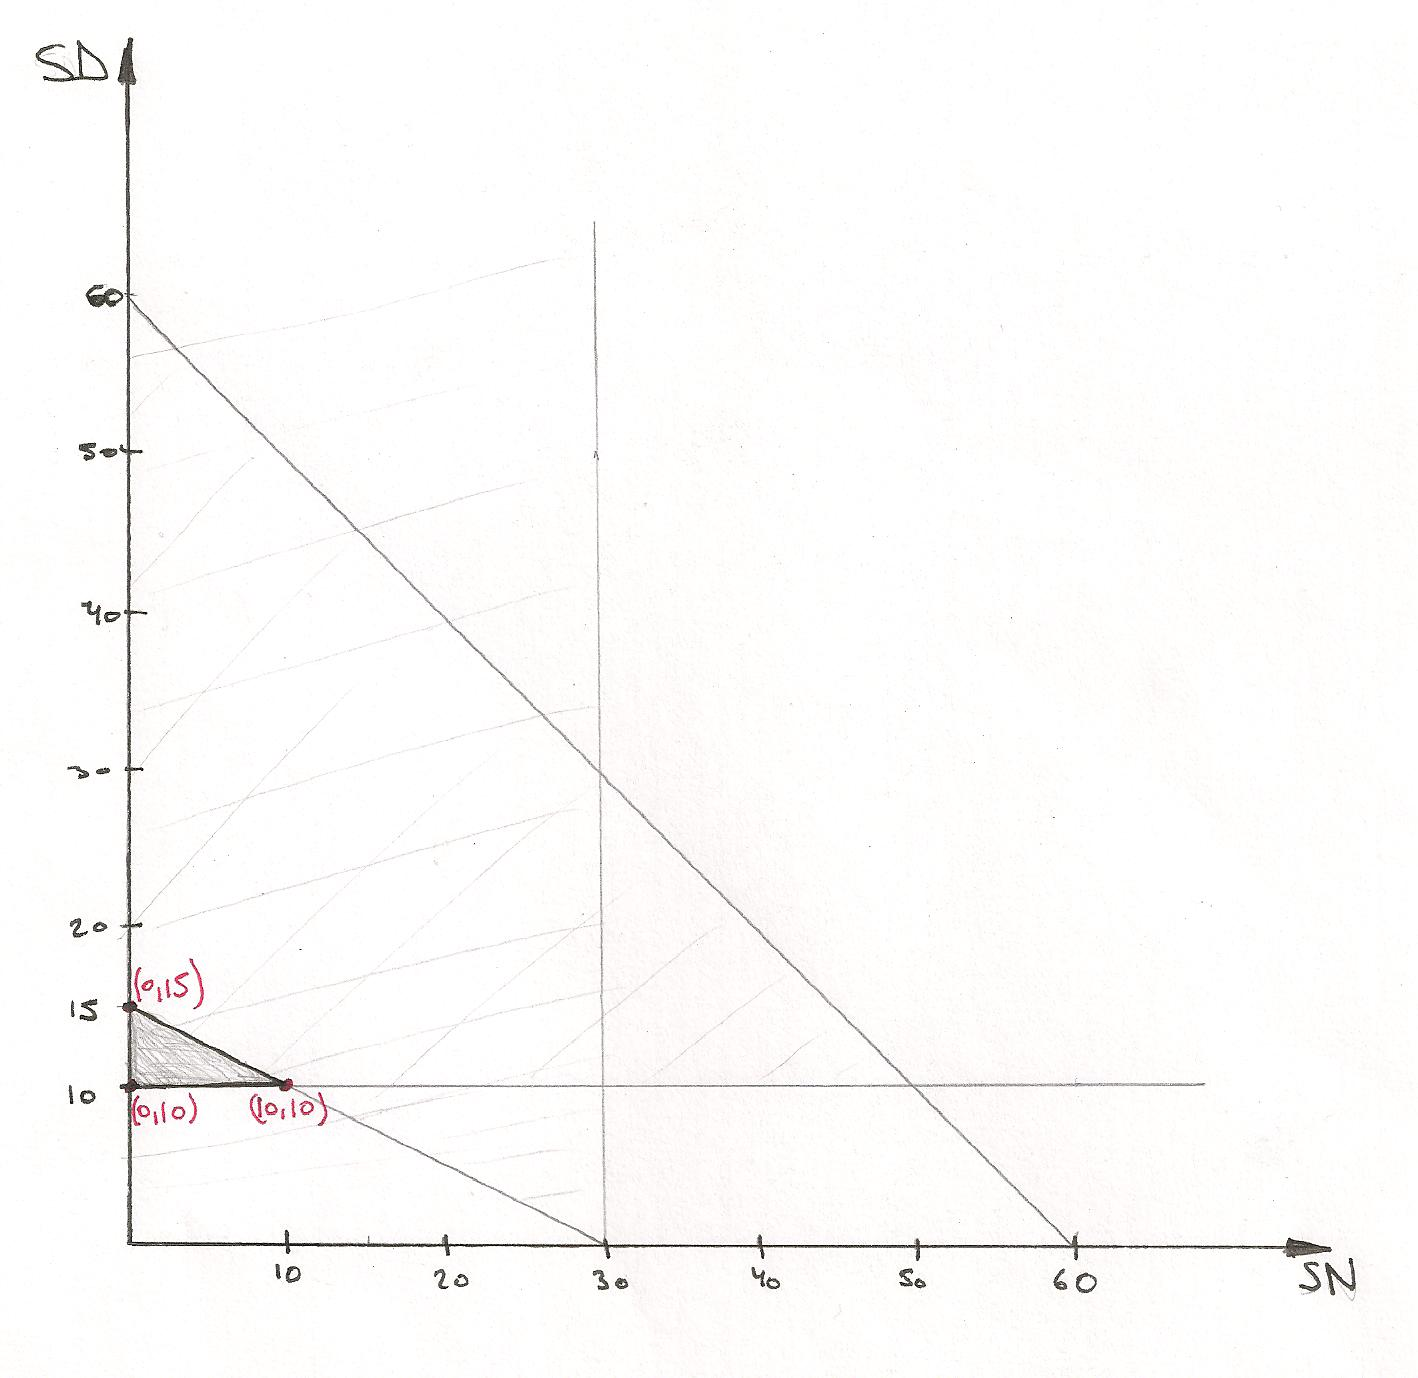
\includegraphics[scale=0.6]{graficoModelos.jpg}
\end{figure}


\subsection{An\'alisis de los Resultados}

Al observar los resultados obtenidos, vemos que la soluci\'on llega a la igualdad de producci\'on tanto de Sidra Dulce como Natural, pero esto no implica que sean igual de \'utiles a la hora de mejorar el funcional. Lo primero que se busc\'o fue cumplir con la condici\'on de compromiso de entrega, obteniendo entonces un m\'inimo de 10 litros de Sidra Dulce. Una vez cubierto este minimo, todos los recursos sobrantes fueron utilizados para producir Sidra Natural, debido a su mayor costo de venta en el mercado.\\

En los valores marginales se puede ver que, si tuviesemos un m\'inimo de 11 para la Sidra Dulce, se obtendr\'ian \$25 menos de beneficio en el funcional ya que el el recurso utilizado ya no estar\'ia disponible para la producci\'on de la Sidra Natural. Bajo el mismo an\'alisis, conseguir un kilo de manzana Verde adicional (ignorando el costo del mismo), implicar\'ia un aumento de \$40 en el funcional, es decir, se obtendr\'ia un mayor beneficio.


\newpage

\section{Anexo I: Modelizaci\'on Ejercicio 1 con GLPK}

\begin{verbatim}
# Resolucion TP - Modelos y Optimizacion I - Catedra Sabados
# Bogado Sebastian 	 - 91707
# Garcia Marra Alejandro - 91516
# Ejercicio 1 - 2da Entrega

			/* variables  */

# Compra
var C1 >= 0;
var C2 >= 0;


# Destilado
var NL >= 0; 
var NLREF >= 0; 
var NLPR >= 0; 
var NLSU >= 0;

var NM >= 0; 
var NMREF >= 0;
var NMPR >= 0;  
var NMSU >= 0; 

var NP >= 0;  
var NPREF >= 0; 
var NPPR >= 0; 
var NPSU >= 0;

var AL >= 0;  
var ALAV >= 0;  
var ALGCRA >= 0;  
var ALACRA >= 0;  
var ALFO >= 0;  

var AP >= 0;  
var APAV >= 0;  
var APGCRA >= 0;  
var APACRA >= 0;  
var APFO >= 0;  

var RDES >= 0;
var RDESAV >= 0;
var RDESLU >= 0;
var RDESFO >= 0; 


# Reformado
var GREF >= 0;
var GREFPR >= 0;
var GREFSU >= 0;


# Craqueo
var GCRA >= 0;
var GCRAPR >= 0;
var GCRASU >= 0;

var ACRA >= 0;
var ACRAAV >= 0;
var ACRAFO >= 0;


# Ventas

var PR >= 0;
var SU >= 0;
var AV >= 0;
var FO >= 0;
var LU >= 0;

/* Funcional */
maximize Z: 700 * PR + 600 * SU + 400 * AV + 350 * FO + 150 * LU;

			/*** Ecuaciones ***/

/*- Destilado -*/

/*Nafta Liviana*/
s.t. inProduccionNL:   NL = 0.1 * C1 + 0.15 * C2;
s.t. outProduccionNL:  NL = NLREF + NLPR + NLSU;

/*Nafta Mediana*/
s.t. inProduccionNM:   NM = 0.2 * C1 + 0.25 * C2;
s.t. outProduccionNM:  NM = NMREF + NMPR + NMSU;

/*Nafta Pesada*/
s.t. inProduccionNP:   NP = 0.2 * C1 + 0.18 * C2;
s.t. outProduccionNP:  NP = NPREF + NPPR + NPSU;

/*Aceite Liviano*/
s.t. inProduccionAL:   AL = 0.12 * C1 + 0.08 * C2;
s.t. outProduccionAL : AL = ALAV + ALGCRA + ALACRA + ALFO;

/*Aceite Pesado*/
s.t. inProduccionAP:   AP = 0.1 * C1;
s.t. outProduccionAP:  AP = APAV + APGCRA + APACRA + APFO;


/*Residuo Destilado*/
s.t. inProduccionRDES:   RDES = 0.13 * C1 + 0.12 * C2;
s.t. outProduccionRDES:  RDES = RDESAV + RDESLU + RDESFO;


/*- Reformado -*/

/*Gasolina Reformada*/
s.t. inProduccionGREF:   GREF = 0.6 * NLREF + 0.52 * NMREF + 0.45 * NPREF;
s.t. outProduccionGREF:  GREF = GREFPR + GREFSU;


/*- Craqueo -*/

/*Gasolina Craqueada*/
s.t. inProduccionGCRA:   GCRA = 0.28 * ALGCRA + 0.2 * APGCRA;
s.t. outProduccionGCRA:  GCRA = GCRAPR + GCRASU;

/*Aceite Craqueado*/
s.t. inProduccionACRA:   ACRA = 0.68 * ALACRA + 0.75 * APACRA;
s.t. outProduccionACRA:  ACRA = ACRAAV + ACRAFO;


/*- Ventas -*/

s.t. finalPR: PR = NLPR + NMPR + NPPR + GCRAPR + GREFPR;
s.t. finalSU: SU = NLSU + NMSU + NPSU + GCRASU + GREFSU;

s.t. ALpartFO: 	 1.8 * FO = ALFO;
s.t. APpartFO: 	   6 * FO = APFO;
s.t. ACRApartFO: 4.5 * FO = ACRAFO;
s.t. RDESpartFO:  18 * FO = RDESFO;

s.t. finalAV: AV = ALAV + APAV + ACRAAV + RDESAV;
s.t. finalLU: LU = RDESLU;


			/** Restricciones **/

			
/* Destilaciones máximas de Crudos */
s.t. dispCrudo1: C1 <= 20000;
s.t. dispCrudo2: C2 <= 30000;
s.t. maxDestilado: C1 + C2 <= 45000;


/* Reformado maximo de naftas */
s.t. maxReformado: NLREF + NMREF + NPREF <= 10000;


/* Craqueo maximo de aceites */
s.t. maxCraqueo: ALGCRA + ALACRA + APGCRA + APACRA <= 8000;


/* Produccion de Lubricantes */
s.t. minLub: LU >= 500;
s.t. maxLub: LU <= 1000;


/* Minimo inProduccion nafta Premium */
s.t. minPremium: PR >= 0.4 * SU;


/* Octanaje nafta Premium */
s.t. minOCTPR: PR * 98 <= 100 * NLPR + 90 * NMPR + 80 * NPPR +
			  + 115 * GCRAPR + 125* GREFPR;

/* Octanaje nafta Super*/
s.t. minOCTSU: SU * 95 <= 100 * NLSU + 90 * NMSU + 80 * NPSU +
			  + 115 * GCRASU + 125* GREFSU;
s.t. maxOCTSU: SU * 97.99 >= 100 * NLSU + 90 * NMSU + 80 * NPSU +
			      + 115 * GCRASU + 125* GREFSU;

			      
/* Presion por cm^2 de Combustible para Aviones*/
s.t. maxPresAV: AV  >= 1 * ALAV + 0.6 * APAV + 1.5 * ACRAAV +
			+ 0.05 * RDESAV;
end;
\end{verbatim}

 \newpage

\section{Anexo II: Modelizaci\'on Ejercicio 2 con GLPK}

 \begin{verbatim}

# Resolucion TP - Modelos y Optimizacion I - Catedra Sabados
# Bogado Sebastian 	 - 91707
# García Marra Alejandro - 91516
# Ejercicio 2 - 2da Entrega

/* variables  */
var SN >= 0;
var SD >= 0;

/* funcional */
maximize Z: 20* SN + 15 * SD;  

/* Restricciones */
s.t. verde: 0.5 * SN + 1 * SD <=15;
s.t. rojas: 1 * SN + 1 * SD <= 60;
s.t. amarillas: 0.5 * SN <= 15;
s.t. reqBar: SD >= 10;

 \end{verbatim}


\end{document}
